\chapter{Statistical analysis of galaxies from a cosmological simulation}
The analysis of the statistical spectrum of distant galaxies may shed light on the properties as well as the inherent history of the universe. Here, a subhalo of a galaxy is analysed 
\begin{equation}
    \delta_{ij} = \frac{n_{ij}-\overline{n}}{\overline{n}}
\end{equation}
\begin{figure}
    \centering
    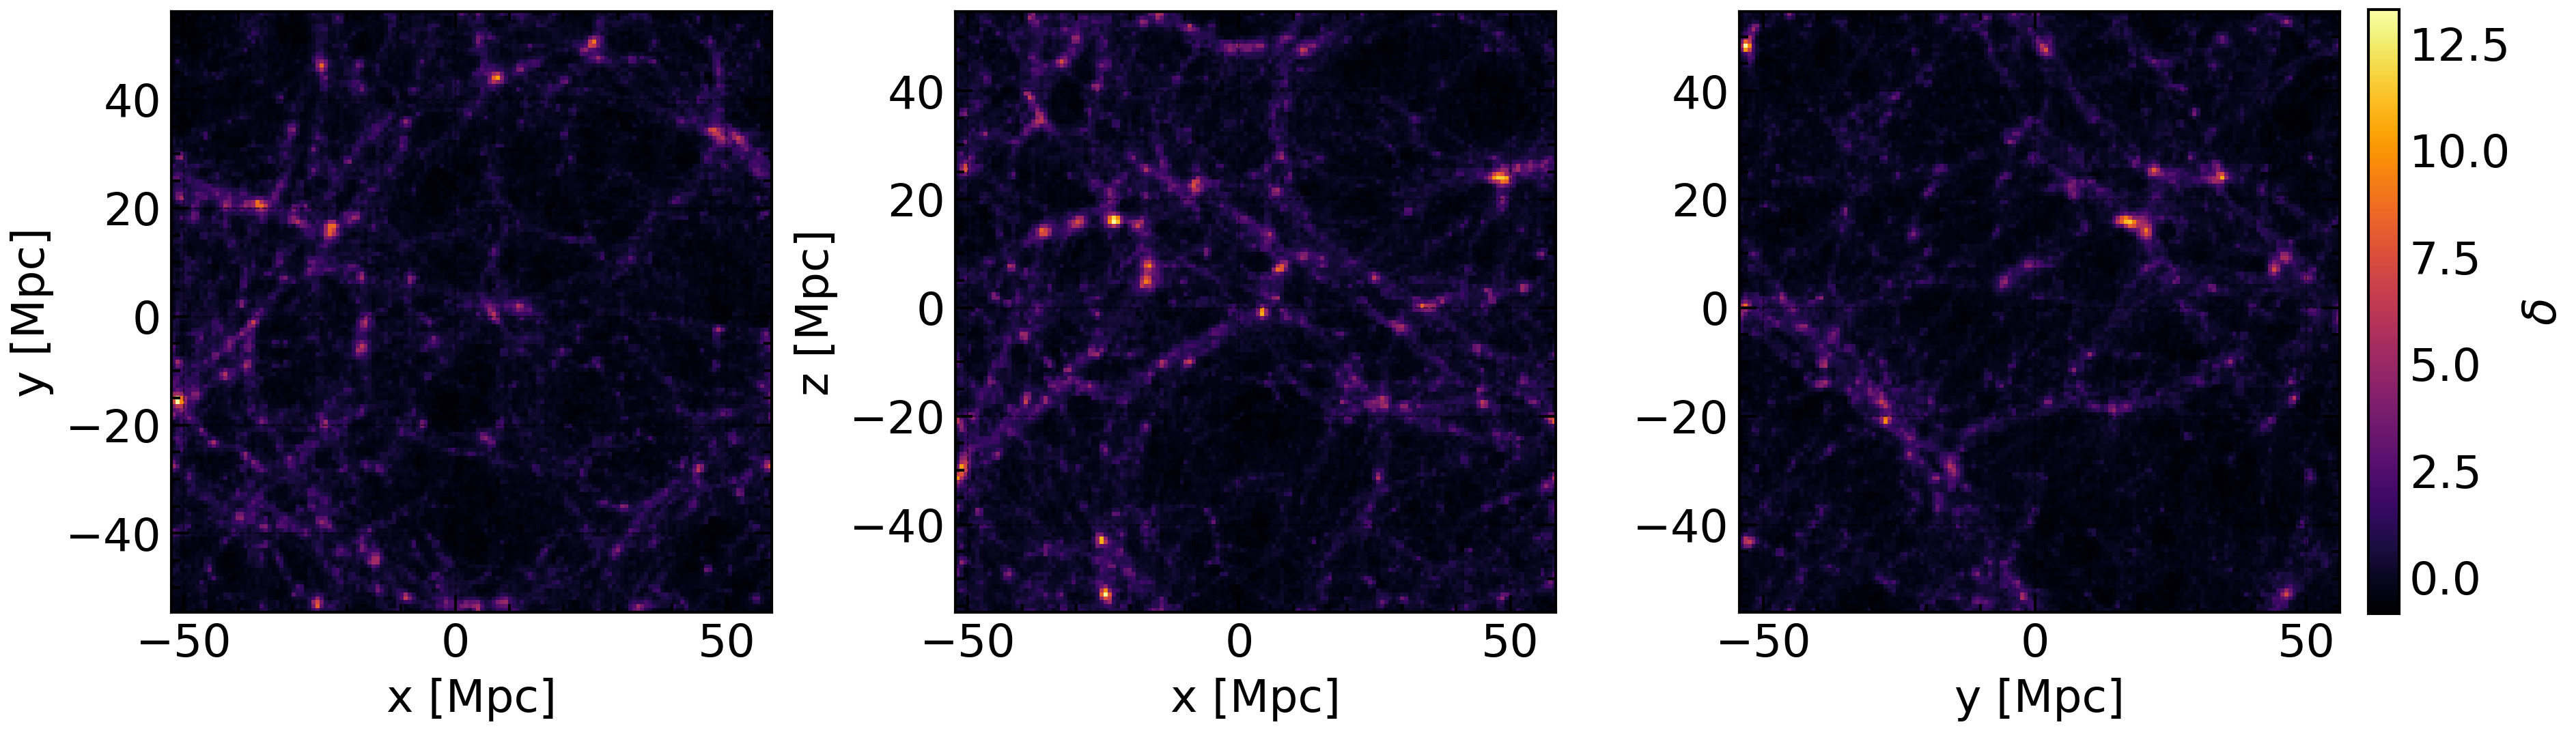
\includegraphics[width=\linewidth]{Figures/Subhalo_density_contrast.png}
    \caption{Density contrast of a subhalo extracted from the TNG100 data set. The three panels show the density contrast in the xy-, xz- and yz- planes respectively. The color bar indicates the value of the density contrast $\delta$. Above distributions of $\delta$ resembles all subhalos in the TNG100 simulation box, whether they host a galaxy or not.}
    \label{fig:placeholder}
\end{figure}
\\
natural estimator
\begin{equation}
    \xi(r) = \frac{\text{DD(r)}}{\text{RR(r)}} - 1
\end{equation}
\begin{equation}
    RR(r) = \frac{N(N-1)}{2V}\cdot\frac{V_\text{shell}}{V}
\end{equation}
\begin{equation}
    \xi(r) = \left(\frac{r}{r_0}\right)^{-\gamma}
\end{equation}
\\
\begin{equation}
    f_\text{b} = \frac{\text{M}_\text{b}}{\text{M}_{\text{vir}}}
\end{equation}
\begin{figure}[htb]
    \centering
    \begin{minipage}{0.45\textwidth}
        \centering
        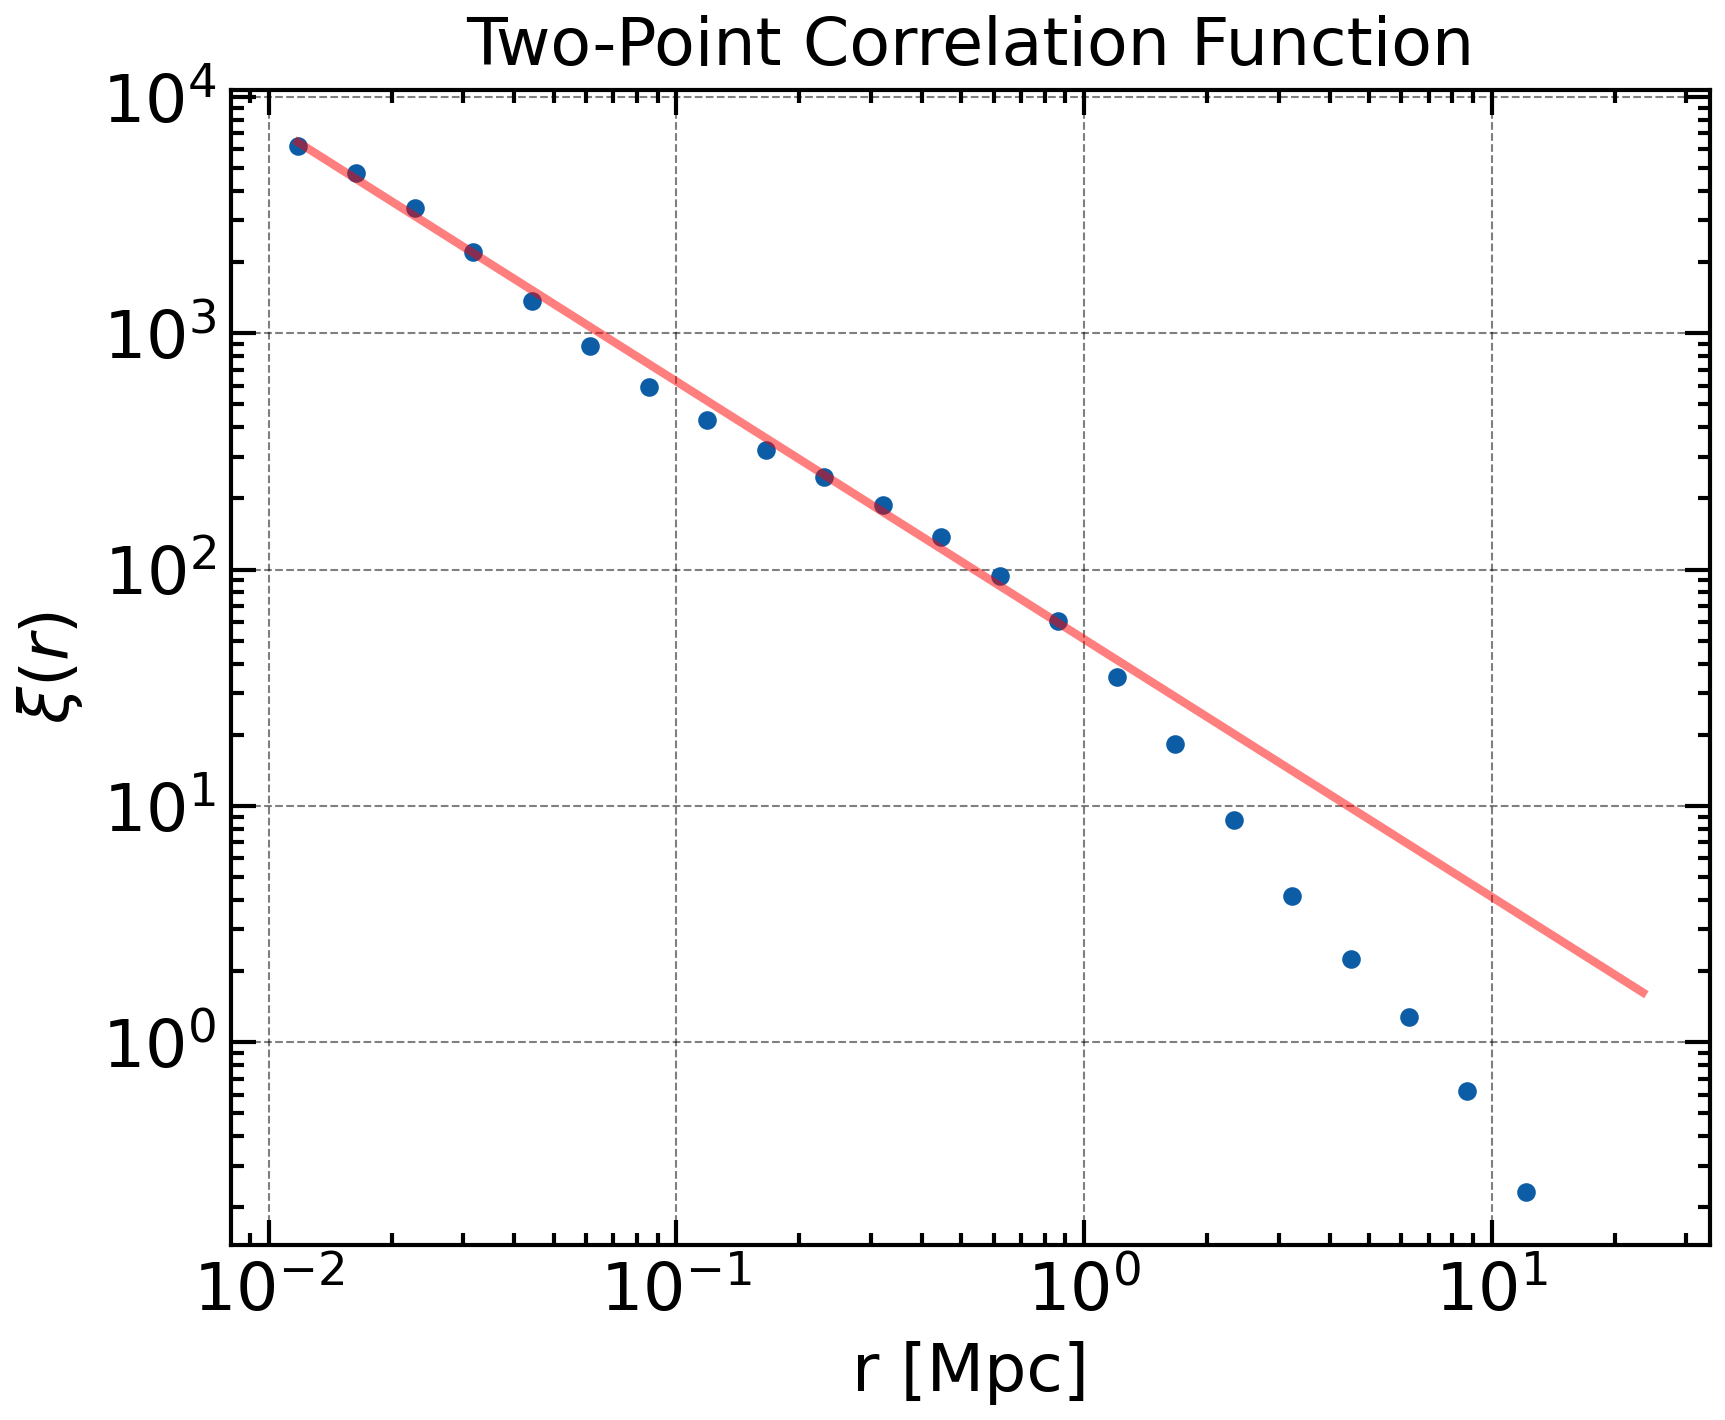
\includegraphics[width=\textwidth]{Figures/Two_Point_Correlation.png}
        \caption{Two-point correlation function $\xi(r)$ of subhalos hosting galaxies. The red line indicates a power-law fit to the data points, with parameters $r_0 = 36.60$ Mpc and $\gamma = 1.09$. Deviation from the power-law for $r \approxeq 1$ Mpc can be observed.}
        \label{fig:two_point_correlation}
    \end{minipage}
    \hfill
    \begin{minipage}{0.45\textwidth}
        \centering
        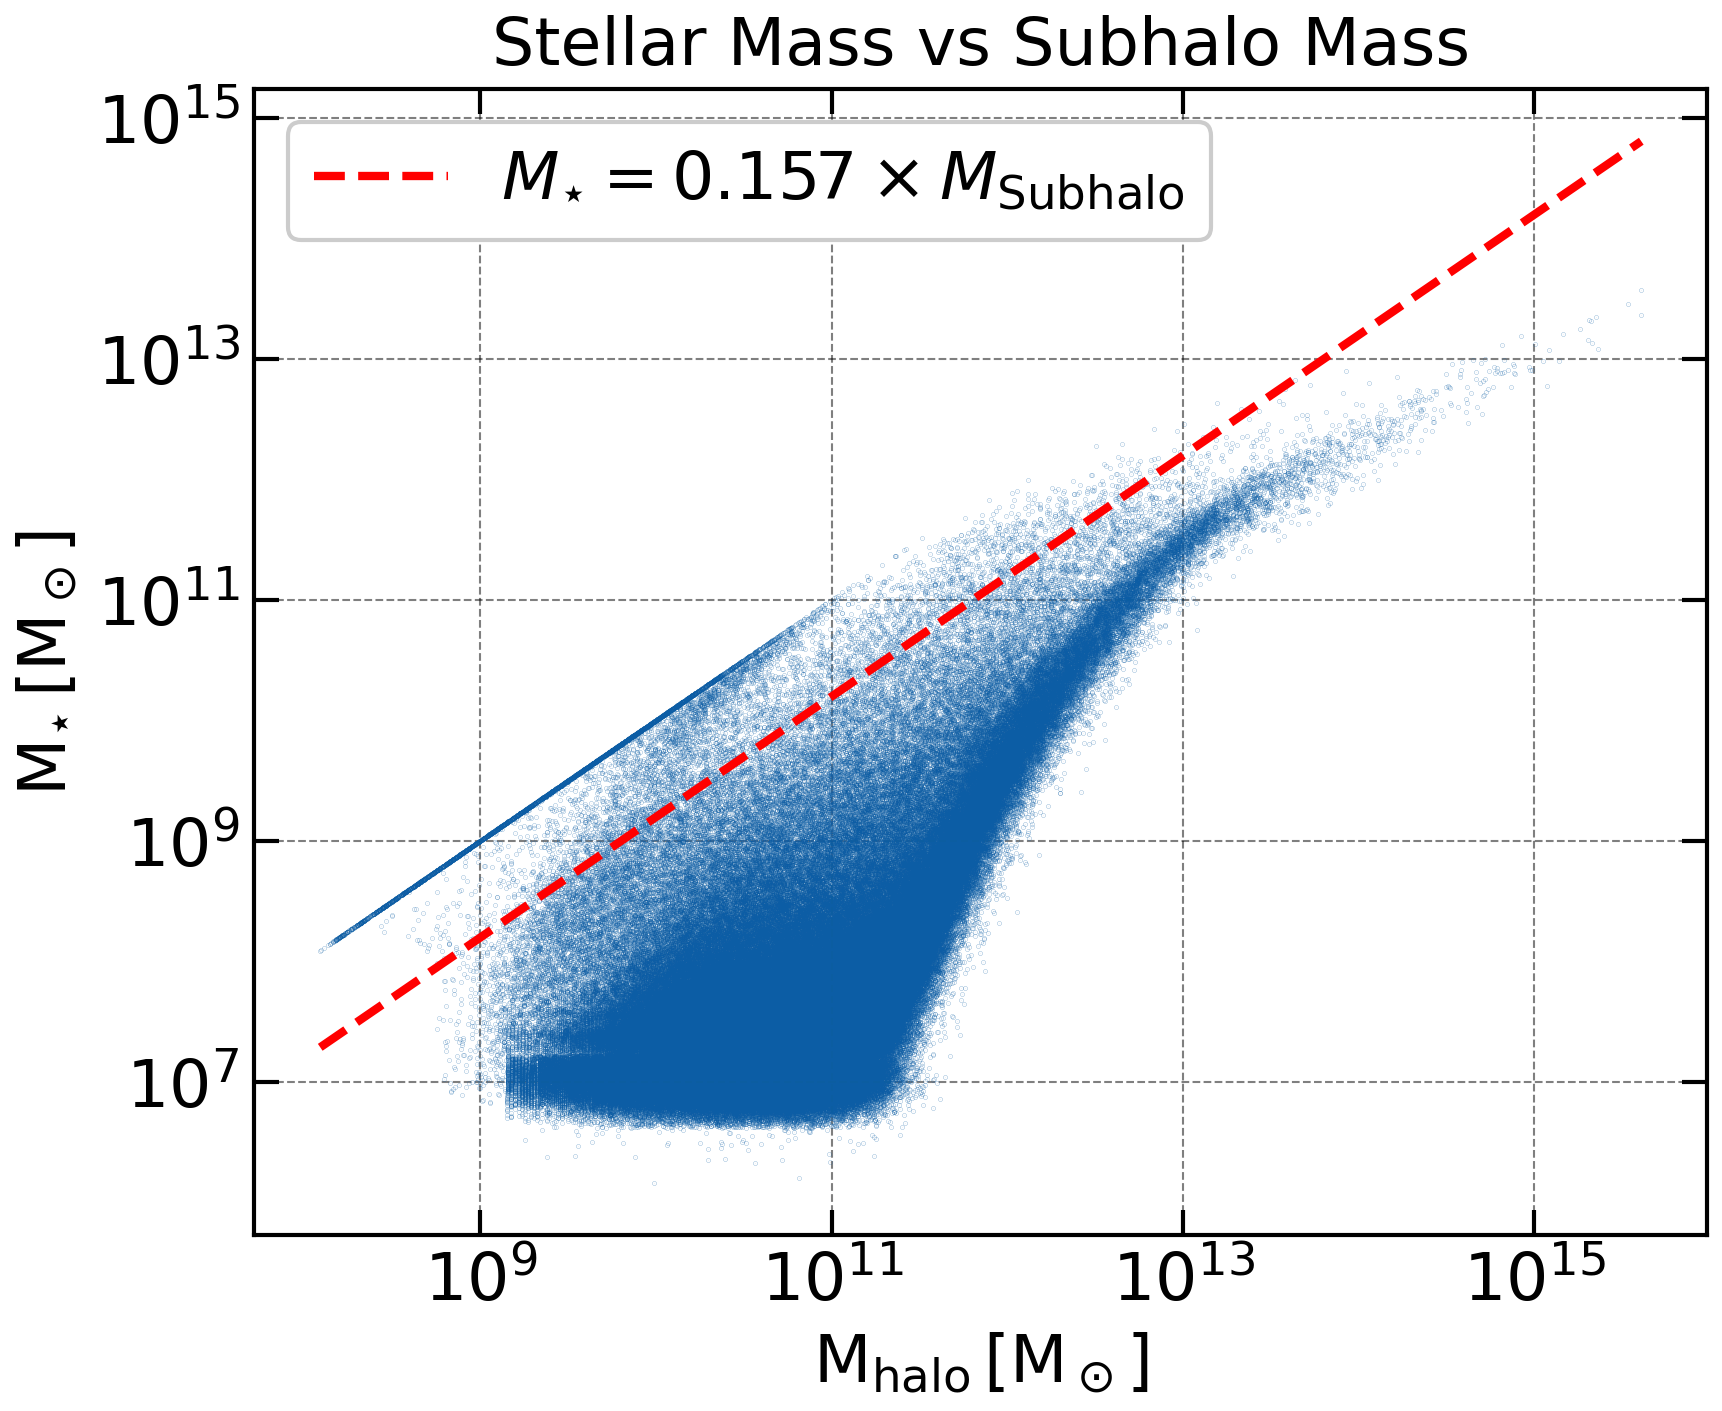
\includegraphics[width=\textwidth]{Figures/Subhalo_Stellar_Mass_vs_subhalo_Mass.png}
        \caption{Scattered stellar mass vs subhalo mass. The red dashed line indicates a linear relation with a slope of $f_\text{b} = 0.157$. The expresses a theoretical upper limit for the stellar mass that can be contained in a halo. Here it can be observed that some subhalos host galaxies with stellar mass exceeding this limit.}
        \label{fig:stellar_vs_subhalo_mass}
    \end{minipage}
\end{figure}


